\documentclass[journal,12pt,twocolumn]{IEEEtran}
%
\usepackage{setspace}
\usepackage{gensymb}
%\doublespacing
\singlespacing

%\usepackage{graphicx}
%\usepackage{amssymb}
%\usepackage{relsize}
\usepackage[cmex10]{amsmath}
\usepackage{siunitx}
%\usepackage{amsthm}
%\interdisplaylinepenalty=2500
%\savesymbol{iint}
%\usepackage{txfonts}
%\restoresymbol{TXF}{iint}
%\usepackage{wasysym}
\usepackage{amsthm}
%\usepackage{iithtlc}
\usepackage{mathrsfs}
\usepackage{txfonts}
\usepackage{stfloats}
\usepackage{steinmetz}
\usepackage{supertabular}
%\usepackage{bm}
\usepackage{cite}
\usepackage{cases}
\usepackage{subfig}
%\usepackage{xtab}
\usepackage{longtable}
\usepackage{multirow}
%\usepackage{algorithm}
%\usepackage{algpseudocode}
\usepackage{enumitem}
\usepackage{mathtools}
\usepackage{tikz}
\usepackage{circuitikz}
\usepackage{verbatim}
\usepackage{tfrupee}
\usepackage[breaklinks=true]{hyperref}
%\usepackage{stmaryrd}
\usepackage{tkz-euclide} % loads  TikZ and tkz-base
%\usetkzobj{all}
\usepackage{pgfplots}
%\usetikzlibrary{all}
\usetikzlibrary{calc,math}
\usetikzlibrary{fadings}
\usetikzlibrary{automata, positioning, arrows}
\usepackage{listings}
    \usepackage{color}                                            %%
    \usepackage{array}                                            %%
    \usepackage{longtable}                                        %%
    \usepackage{calc}                                             %%
    \usepackage{multirow}                                         %%
    \usepackage{hhline}                                           %%
    \usepackage{ifthen}                                           %%
  %optionally (for landscape tables embedded in another document): %%
    \usepackage{lscape}     
\usepackage{multicol}
\usepackage{chngcntr}
\usepackage{blkarray}
%\usepackage{enumerate}

%\usepackage{wasysym}
%\newcounter{MYtempeqncnt}
\DeclareMathOperator*{\Res}{Res}
%\renewcommand{\baselinestretch}{2}
\renewcommand\thesection{\arabic{section}}
\renewcommand\thesubsection{\thesection.\arabic{subsection}}
\renewcommand\thesubsubsection{\thesubsection.\arabic{subsubsection}}

\renewcommand\thesectiondis{\arabic{section}}
\renewcommand\thesubsectiondis{\thesectiondis.\arabic{subsection}}
\renewcommand\thesubsubsectiondis{\thesubsectiondis.\arabic{subsubsection}}

% correct bad hyphenation here
\hyphenation{op-tical net-works semi-conduc-tor}
\def\inputGnumericTable{}                                 %%

\lstset{
%language=C,
frame=single, 
breaklines=true,
columns=fullflexible
}
%\lstset{
%language=tex,
%frame=single, 
%breaklines=true
%}

\begin{document}
%


\newtheorem{theorem}{Theorem}[section]
\newtheorem{problem}{Problem}
\newtheorem{proposition}{Proposition}[section]
\newtheorem{lemma}{Lemma}[section]
\newtheorem{corollary}[theorem]{Corollary}
\newtheorem{example}{Example}[section]
\newtheorem{definition}[problem]{Definition}
%\newtheorem{thm}{Theorem}[section] 
%\newtheorem{defn}[thm]{Definition}
%\newtheorem{algorithm}{Algorithm}[section]
%\newtheorem{cor}{Corollary}
\newcommand{\BEQA}{\begin{eqnarray}}
\newcommand{\EEQA}{\end{eqnarray}}
\newcommand{\define}{\stackrel{\triangle}{=}}

\bibliographystyle{IEEEtran}
%\bibliographystyle{ieeetr}


\providecommand{\mbf}{\mathbf}
\providecommand{\pr}[1]{\ensuremath{\Pr\left(#1\right)}}
\providecommand{\qfunc}[1]{\ensuremath{Q\left(#1\right)}}
\providecommand{\sbrak}[1]{\ensuremath{{}\left[#1\right]}}
\providecommand{\lsbrak}[1]{\ensuremath{{}\left[#1\right.}}
\providecommand{\rsbrak}[1]{\ensuremath{{}\left.#1\right]}}
\providecommand{\brak}[1]{\ensuremath{\left(#1\right)}}
\providecommand{\lbrak}[1]{\ensuremath{\left(#1\right.}}
\providecommand{\rbrak}[1]{\ensuremath{\left.#1\right)}}
\providecommand{\cbrak}[1]{\ensuremath{\left\{#1\right\}}}
\providecommand{\lcbrak}[1]{\ensuremath{\left\{#1\right.}}
\providecommand{\rcbrak}[1]{\ensuremath{\left.#1\right\}}}
\theoremstyle{remark}
\newtheorem{rem}{Remark}
\newcommand{\sgn}{\mathop{\mathrm{sgn}}}
\providecommand{\abs}[1]{\left\vert#1\right\vert}
\providecommand{\res}[1]{\Res\displaylimits_{#1}} 
\providecommand{\norm}[1]{\left\lVert#1\right\rVert}
%\providecommand{\norm}[1]{\lVert#1\rVert}
\providecommand{\mtx}[1]{\mathbf{#1}}
\providecommand{\mean}[1]{E\left[ #1 \right]}
\providecommand{\fourier}{\overset{\mathcal{F}}{ \rightleftharpoons}}
%\providecommand{\hilbert}{\overset{\mathcal{H}}{ \rightleftharpoons}}
\providecommand{\system}{\overset{\mathcal{H}}{ \longleftrightarrow}}
	%\newcommand{\solution}[2]{\textbf{Solution:}{#1}}
\newcommand{\solution}{\noindent \textbf{Solution: }}
\newcommand{\cosec}{\,\text{cosec}\,}
\providecommand{\dec}[2]{\ensuremath{\overset{#1}{\underset{#2}{\gtrless}}}}
\newcommand{\myvec}[1]{\ensuremath{\begin{pmatrix}#1\end{pmatrix}}}
\newcommand{\mydet}[1]{\ensuremath{\begin{vmatrix}#1\end{vmatrix}}}
\newcommand*{\permcomb}[4][0mu]{{{}^{#3}\mkern#1#2_{#4}}}
\newcommand*{\perm}[1][-3mu]{\permcomb[#1]{P}}
\newcommand*{\comb}[1][-1mu]{\permcomb[#1]{C}}
\newcommand{\Int}{\int\limits}

%\numberwithin{equation}{section}
\numberwithin{equation}{subsection}
%\numberwithin{problem}{section}
%\numberwithin{definition}{section}
\makeatletter
\@addtoreset{figure}{problem}
\makeatother

\let\StandardTheFigure\thefigure
\let\vec\mathbf
%\renewcommand{\thefigure}{\theproblem.\arabic{figure}}
\renewcommand{\thefigure}{\theproblem}
%\setlist[enumerate,1]{before=\renewcommand\theequation{\theenumi.\arabic{equation}}
%\counterwithin{equation}{enumi}


%\renewcommand{\theequation}{\arabic{subsection}.\arabic{equation}}

\def\putbox#1#2#3{\makebox[0in][l]{\makebox[#1][l]{}\raisebox{\baselineskip}[0in][0in]{\raisebox{#2}[0in][0in]{#3}}}}
     \def\rightbox#1{\makebox[0in][r]{#1}}
     \def\centbox#1{\makebox[0in]{#1}}
     \def\topbox#1{\raisebox{-\baselineskip}[0in][0in]{#1}}
     \def\midbox#1{\raisebox{-0.5\baselineskip}[0in][0in]{#1}}

\vspace{3cm}

\title{
%	\logo{
Probability
%	}
}
\author{ G V V Sharma$^{*}$% <-this % stops a space
	\thanks{*The author is with the Department
		of Electrical Engineering, Indian Institute of Technology, Hyderabad
		502285 India e-mail:  gadepall@iith.ac.in. All content in this manual is released under GNU GPL.  Free and open source.}
	
}	
%\title{
%	\logo{Matrix Analysis through Octave}{\begin{center}\includegraphics[scale=.24]{tlc}\end{center}}{}{HAMDSP}
%}


% paper title
% can use linebreaks \\ within to get better formatting as desired
%\title{Matrix Analysis through Octave}
%
%
% author names and IEEE memberships
% note positions of commas and nonbreaking spaces ( ~ ) LaTeX will not break
% a structure at a ~ so this keeps an author's name from being broken across
% two lines.
% use \thanks{} to gain access to the first footnote area
% a separate \thanks must be used for each paragraph as LaTeX2e's \thanks
% was not built to handle multiple paragraphs
%

%\author{<-this % stops a space
%\thanks{}}
%}
% note the % following the last \IEEEmembership and also \thanks - 
% these prevent an unwanted space from occurring between the last author name
% and the end of the author line. i.e., if you had this:
% 
% \author{....lastname \thanks{...} \thanks{...} }
%                     ^------------^------------^----Do not want these spaces!
%
% a space would be appended to the last name and could cause every name on that
% line to be shifted left slightly. This is one of those "LaTeX things". For
% instance, "\textbf{A} \textbf{B}" will typeset as "A B" not "AB". To get
% "AB" then you have to do: "\textbf{A}\textbf{B}"
% \thanks is no different in this regard, so shield the last } of each \thanks
% that ends a line with a % and do not let a space in before the next \thanks.
% Spaces after \IEEEmembership other than the last one are OK (and needed) as
% you are supposed to have spaces between the names. For what it is worth,
% this is a minor point as most people would not even notice if the said evil
% space somehow managed to creep in.



% The paper headers
%\markboth{Journal of \LaTeX\ Class Files,~Vol.~6, No.~1, January~2007}%
%{Shell \MakeLowercase{\textit{et al.}}: Bare Demo of IEEEtran.cls for Journals}
% The only time the second header will appear is for the odd numbered pages
% after the title page when using the twoside option.
% 
% *** Note that you probably will NOT want to include the author's ***
% *** name in the headers of peer review papers.                   ***
% You can use \ifCLASSOPTIONpeerreview for conditional compilation here if
% you desire.




% If you want to put a publisher's ID mark on the page you can do it like
% this:
%\IEEEpubid{0000--0000/00\$00.00~\copyright~2007 IEEE}
% Remember, if you use this you must call \IEEEpubidadjcol in the second
% column for its text to clear the IEEEpubid mark.



% make the title area
\maketitle

%\newpage

\tableofcontents

\newpage

\bigskip

\renewcommand{\thefigure}{\theenumi}
\renewcommand{\thetable}{\theenumi}
%\renewcommand{\theequation}{\theenumi}

%\begin{abstract}
%%\boldmath
%In this letter, an algorithm for evaluating the exact analytical bit error rate  (BER)  for the piecewise linear (PL) combiner for  multiple relays is presented. Previous results were available only for upto three relays. The algorithm is unique in the sense that  the actual mathematical expressions, that are prohibitively large, need not be explicitly obtained. The diversity gain due to multiple relays is shown through plots of the analytical BER, well supported by simulations. 
%
%\end{abstract}
% IEEEtran.cls defaults to using nonbold math in the Abstract.
% This preserves the distinction between vectors and scalars. However,
% if the journal you are submitting to favors bold math in the abstract,
% then you can use LaTeX's standard command \boldmath at the very start
% of the abstract to achieve this. Many IEEE journals frown on math
% in the abstract anyway.

% Note that keywords are not normally used for peerreview papers.
%\begin{IEEEkeywords}
%Cooperative diversity, decode and forward, piecewise linear
%\end{IEEEkeywords}



% For peer review papers, you can put extra information on the cover
% page as needed:
% \ifCLASSOPTIONpeerreview
% \begin{center} \bfseries EDICS Category: 3-BBND \end{center}
% \fi
%
% For peerreview papers, this IEEEtran command inserts a page break and
% creates the second title. It will be ignored for other modes.
%\IEEEpeerreviewmaketitle

\begin{abstract}
This book provides solved examples on Probability
\end{abstract}

\section{Axioms of Probability}
\renewcommand{\theequation}{\theenumi}
\renewcommand{\thefigure}{\theenumi}
\renewcommand{\thetable}{\theenumi}
\begin{enumerate}[label=\thesection.\arabic*.,ref=\thesection.\theenumi]
\numberwithin{equation}{enumi}
\numberwithin{figure}{enumi}
\numberwithin{table}{enumi}

\item The probability that a given positive integer lying between 1 and 100 (both inclusive) is NOT divisible by 2,3 or 5 is \dots
\\
\solution
Table \ref{gate:11} summarizes the given information. 
\begin{table}[!ht]
    \begin{center}
        \renewcommand{\arraystretch}{2.5}
    \begin{tabular}{|c|c|c|}
    \hline
    Event & Definition & Probability  \\
    \hline
    A    & $n \equiv 0 \pmod{2}$  & $\cfrac{50}{100}$ \\ \hline
    B    & $n \equiv 0 \pmod{3}$ & $\cfrac{33}{100}$ \\ \hline
    C    & $n \equiv 0 \pmod{5}$  & $\cfrac{20}{100}$ \\ \hline
    AB   & $n \equiv 0 \pmod{6}$ & $\cfrac{16}{100}$ \\ \hline
    BC   & $n \equiv 0 \pmod{15}$ & $\cfrac{6}{100}$ \\ \hline
    AC   & $n \equiv 0 \pmod{10}$ & $\cfrac{10}{100}$ \\ \hline
    ABC  & $n \equiv 0 \pmod{30}$ & $\cfrac{3}{100}$ \\
    \hline
    \end{tabular}
    \renewcommand{\arraystretch}{1}
    \end{center}
    \caption{$1 \le n \le 100$}
    \label{gate:11}
    \end{table}
    %
%
\begin{multline}
\because     \pr{A+B+C} = \pr{A} + \pr{B} + \pr{C} \\- \pr{AB} - \pr{BC} \\- \pr{AC} + \pr{ABC}\label{Shurururururururu}    
\end{multline}

Substituting from Table \ref{gate:11} in \eqref{Shurururururururu},
\begin{multline}
    \pr{A+B+C} = \frac{50}{100} + \frac{33}{100} + \frac{20}{100} \\- \frac{16}{100} - \frac{6}{100} - \frac{10}{100} + \frac{3}{100} 
    \\
    = \frac{74}{100}
\end{multline}
Thus, the  required probability is
\begin{align}
    1 - \pr{A+B+C} = \frac{26}{100}
\end{align}

%
\item P and Q are considering to apply for a job. The probability that P applies for the job is $\dfrac{1}{4}$, the probability that P applies for the job given that Q applies for the job is $\dfrac{1}{2}$, and the probability that Q applies for the job given that P applies for the job is $\dfrac{1}{3}$. Then the probability that P does not apply for the job given that Q does not apply for the job is 

\begin{enumerate}
\begin{multicols}{4}
\setlength\itemsep{2em}

\item $
\dfrac{4}{5}
$

\item $
\dfrac{5}{6}
$

\item $
\dfrac{7}{8}
$

\item $
\dfrac{11}{12}
$

\end{multicols}
\end{enumerate}
\solution
The given information can be expressed as
\begin{align}
    \label{eq:axioms/2/given}
    \pr{P} &= \frac{1}{4} \\
    \pr{P|Q} &= \frac{1}{2}  = \frac{\pr{PQ}}{\pr{Q}}\\
    \pr{Q|P} &= \frac{1}{3}  =  \frac{\pr{PQ}}{\pr{P}}
    \end{align}
    which yields
    \begin{align}
        \label{eq:axioms/2/derived}
        \begin{split}
        \pr{PQ} &= \frac{1}{3} \times \frac{1}{4}  = \frac{1}{12}
        \\
        \pr{Q} &= \frac{\frac{1}{12}}{\frac{1}{2}} = \frac{1}{6}
        \end{split}
        \end{align}
    
The objective is to find
\begin{align}
    \pr{P^{\prime}|Q^{\prime}}
    \label{eq:axioms/2/tofind}
\end{align}
\eqref{eq:axioms/2/given} can be expressed as 
\begin{align}
    \pr{P^{\prime}|Q^{\prime}} &= \frac{\pr{P^{\prime}Q^{\prime}}}{\pr{Q^{\prime}}} 
\\
&= \frac{\pr{1 - \brak{P + Q}^{\prime}}}{\pr{Q^{\prime}}} 
\\
&= \frac{1 - \pr{P}-\pr{Q} +\pr{PQ}}{1 - \pr{Q}} 
   \label{2.0.19}   
    \end{align}
Substituting from     \eqref{eq:axioms/2/derived} and     \eqref{eq:axioms/2/given} in    \eqref{2.0.19},   
\begin{align}
    \pr{P^{\prime}|Q^{\prime}} = \frac{4}{5}
\end{align}


%
\item An experiment consists of two papers.paper1 and paper2.The probability of failing in paper 1 is .3 and that in paper 2 is .2.Given that a student has failed in paper 2,the probability of failing in paper 1 is .6.The probability of student failing in both is\\
\begin{enumerate}
    \setlength\itemsep{2em}
\item .5 
\item .18 
\item .12 
\item .06 
\end{enumerate}
%
\solution
\begin{table}[!ht]
    \centering
    \begin{tabular}{|c|c|c|}
    \hline
         &Description  & Probability \\
         \hline
         0&failure & $\pr{X=0} = 0.3$\\
         \hline
         1&success & $\pr{Y=0} = 0.2$\\
         \hline
         X&Paper 1 & $\pr{X=0|Y=0} = 0.6$\\
         \hline
         Y&Paper 2 & \\
         \hline
    \end{tabular}
    \caption{Description}
    \label{table:axioms/3}
\end{table}
%
Table \ref{table:axioms/3} summarises the given information.  The desired probability is
%
    \begin{align}
        \pr{X=0,Y=0} &= \pr{X=0|Y=0}\pr{Y=0}\\ 
        &=.12
       \end{align}

%



\end{enumerate}

\section{Markov Chain}
\renewcommand{\theequation}{\theenumi}
\renewcommand{\thefigure}{\theenumi}
\renewcommand{\thetable}{\theenumi}
\begin{enumerate}[label=\thesection.\arabic*.,ref=\thesection.\theenumi]
\numberwithin{equation}{enumi}
\numberwithin{figure}{enumi}
\numberwithin{table}{enumi}


\item \textbf{Step 1.} Flip a coin twice.\\
\textbf{Step 2.} If the outcomes are (TAILS, HEADS) then output Y and stop.\\
\textbf{Step 3.} If the outcomes are either (HEADS, HEADS) or (HEADS, TAILS), then output N and stop.\\
\textbf{Step 4.} If the outcomes are (TAILS, TAILS), then go to Step 1.\\
The probability that the output of the experiment is Y is (upto two decimal places)......
%
\solution
Given, a fair coin is tossed is tossed two times.
Let's define a Markov chain $\{X_{n},n=0,1,2,\dots\}$, where $X_{n}\in S=\{1,2,3\}$, such that
\begin{table}[h!]
\centering
\caption{States and their notations}
\label{ec9:table:1}
\begin{tabular}{|c|c|}
    \hline
    Notation & State \\
    \hline
    $S=1$ & getting \cbrak{TT}\\[1ex]
    \hline
    $S=2$ & getting output Y\\[1ex]
    \hline
    $S=3$ & getting output N\\[1ex]
    \hline
\end{tabular}
\end{table}\\
The state transition matrix for the Markov chain is
\begin{align}
\label{ec9:eq:1}
P=\begin{blockarray}{cccccc}
&1 & 2 & 3 \\
\begin{block}{c[ccccc]}
  1 & 0.25 & 0.25 & 0.5  \\
  2 & 0 & 1 & 0 \\
  3 & 0 & 0 & 1  \\
\end{block}
\end{blockarray}
\end{align}
Clearly, the state $1$ are transient, while $2,3$ are absorbing. The standard form of a state transition matrix is
\begin{align}
\label{ec9:eq:2}
P=\begin{blockarray}{ccc}
&A & N \\
\begin{block}{c[cc]}
  A & I & O  \\
  N & R & Q \\
\end{block}
\end{blockarray}
\end{align}
where,
\begin{table}[h!]
\centering
\caption{Notations and their meanings}
\label{ec9:table:2}
\begin{tabular}{|c|c|}
    \hline
    Notation & Meaning \\
    \hline
    $A$ & All absorbing states\\[1ex]
    \hline
    $N$ & All non-absorbing states\\[1ex]
    \hline
    $I$ & Identity matrix\\[1ex]
    \hline
    $O$ & Zero matrix\\[1ex]
    \hline
    $R,Q$ & Other submatices\\[1ex]
    \hline
\end{tabular}
\end{table}
Converting \eqref{ec9:eq:1} to standard form, we get
\begin{align}
P=\begin{blockarray}{cccccc}
&2 & 3 & 1  \\
\begin{block}{c[ccccc]}
  2 & 1 & 0 & 0  \\
  3 & 0 & 1 & 0 \\
  1 & 0.25 & 0.5 & 0.25  \\
\end{block}
\end{blockarray}
\end{align}
From \eqref{ec9:eq:2},
\begin{align}
\tag{104.5}
\label{ec9:eq:r,q}
    R=\begin{bmatrix}
    0.25 & 0.5\\
    \end{bmatrix},
    Q=\begin{bmatrix}
    0.25\\
    \end{bmatrix}
\end{align}
The limiting matrix for absorbing Markov chain is
\begin{align}
\bar P=\begin{bmatrix}
    I & O\\
    FR & O\\
    \end{bmatrix}
\end{align}
where,
\begin{align}
F=(I-Q)^{-1}
\end{align}
is called the fundamental matrix of $P$. \\
On solving, we get
\begin{align}
\bar P=\begin{blockarray}{cccccc}
&2 & 3 & 1 \\
\begin{block}{c[ccccc]}
    2 & 1 & 0 & 0\\ 
    3 & 0 & 1 & 0\\ 
    1 & 0.33 & 0.17 & 0\\    
\end{block}
\end{blockarray}
\end{align}
A element $\bar p_{ij}$ of $\bar P$ denotes the absorption probability in state $j$, starting from state $i$. 
\\ Then, the absorption probability in state 2 $\brak{\text{i.e getting output Y}}$ starting from state 1 is $\bar p_{12}$.
\begin{align}
\therefore \bar p_{12}=0.33 \brak{\text{correct upto 2 decimal places}}
\end{align}
\begin{figure}[h]
\caption*{\textbf{Markov chain diagram}}
\centering
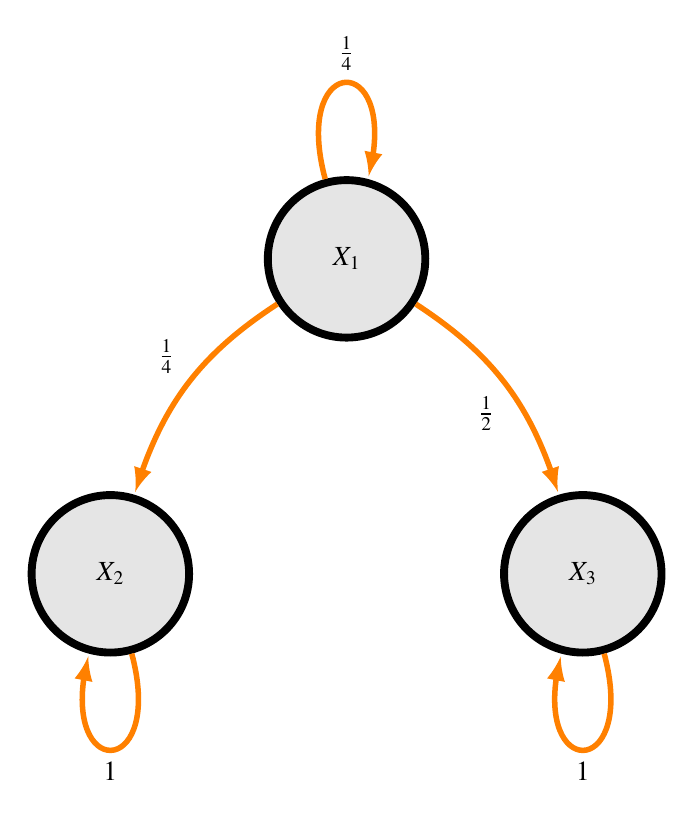
\begin{tikzpicture}
       
             % Setup the style for the states
        \tikzset{node style/.style={state, 
                                    minimum width=2cm,
                                    line width=1mm,
                                    fill=gray!20!white}}
        % Draw the states
        \node[node style] at (3, 0)      (bull)     {$X_{1}$};
        \node[node style] at (0, -4)      (bear)     {$X_{2}$};
        \node[node style] at (6, -4) (stagnant) {$X_{3}$};
        % Connect the states with arrows
        \draw[every loop,
              auto=right,
              line width=0.7mm,
              >=latex,
              draw=orange,
              fill=orange]
           (bull)     edge[bend left=20]            node {$\frac{1}{2}$} (stagnant)
            (bull)     edge[bend right=20] node {$\frac{1}{4}$} (bear)
            
            
            (bull) edge[loop above]             node  {$\frac{1}{4}$} (bull)
            (bear) edge[loop below]             node  {1} (bear)
            (stagnant) edge[loop below]             node  {1} (stagnant);
    \end{tikzpicture}
\end{figure}


\end{enumerate}

%  \section{June 2019}
%  \input{./chapters/2019.tex}
% \section{December 2018}
% \input{./chapters/2018/dec.tex}
% \section{June 2018}
% \input{./chapters/2018/june.tex}
% \section{December 2017}
% \input{./chapters/2017/dec.tex}
% %\twocolumn
% \section{June 2017}
% \input{./chapters/2017/june.tex}
% \section{December 2016}
% \input{./chapters/2016/dec.tex}
% \section{June 2016}
% \input{./chapters/2016/june.tex}
% \section{December 2015}
% \input{./chapters/2015/dec.tex}
% \section{June 2015}
% \input{./chapters/2015/june.tex}
%  \section{December 2014}
%  \input{./chapters/2014/dec.tex}
% \section{June 2013}
% \input{./chapters/2013/june.tex}

% \section{December 2012}
% \input{./chapters/2012/dec.tex}

% \section{June 2012}
% \input{./chapters/2012/june.tex}


\end{document}


